\chapter{The Complementary Filter}
Two different complementary filters were investigated and their responses were modeled in MatLab before they were tested on the Quad-Rotor. This chapter describes in detail these two complementary filters.

\section{ Complementary Filter}
The Complementary filter gets its name from the manner in which the high-pass and low-pass filters which make up the Complementary filter are chosen. Hence, a pair of filters are called complementary filters if their transfer functions sum to one at all frequencies in a complex sense, i.e. the phase is zero and the magnitude is one as seen in following:-

\begin{equation}
	G_1(s) + G_2(s) =1 \label{eq: bases of comp filter1}
\end{equation}



Figure \ref{fig: Block Diagram of First Order Complementary Filter} is a block diagram representation of a first order complementary filter. As can be seen from the figure, the accelerometer data is low pass filtered while the gyroscope data is high pass filtered. The filters used in this report are augmented forms of the filters presented in \cite{sprague2001design,comp_filter_mit}. The first filter that was investigated first and is depicted in figure \ref{fig: Block Diagram of First Order Complementary Filter}.


\tikzset{%
block/.style    = {draw, thick, rectangle, minimum height = 3em,minimum width = 3em},
input/.style    = {coordinate}, % Input
output/.style   = {coordinate} % Output
block/.style    = {draw, thick, rectangle, minimum height = 3em,minimum width = 3em},
gain/.style     = {draw, thick, isosceles triangle, minimum height = 2em,
		isosceles triangle apex angle=60},
port/.style     = {inner sep=0pt, font=\tiny},
sum/.style n args = {4}{draw, circle, node distance = 2cm, minimum size=5mm, alias=sum,
		append after command={
				node at (sum.north) [port, below=1pt] {$#1$}
				node at (sum.west) [port, right=1pt] {$#2$}
				node at (sum.south) [port, above=1pt] {$#3$}
				node at (sum.east) [port, left=1pt] {$#4$}
			},
	}, % Adder
joint/.style    = {circle, draw, fill, inner sep=0pt, minimum size=2pt},
input/.style    = {coordinate}, % Input
output/.style   = {coordinate} % Output
}
% Defining string as labels of certain blocks.
\newcommand{\suma}{\Large$+$}
\newcommand{\inte}{$\displaystyle \int$}
\newcommand{\derv}{\huge$\frac{d}{dt}$}


\begin{figure}[h]
	\centering
	\begin{tikzpicture}[auto, thick, node distance=2cm, >=triangle 45]
		\draw
		% Drawing the blocks of first filter :
		
		node at (0,0) [input,name=input1,thick,above]{}
		node at (4,0)[block] (lpf) {\Large $\frac{1}{1+\tau s}$}
		node at (0,-2) [name=input2] {}
		node at (6,-2) [block](inte1) {\inte}
		node at (4,-2)[block] (hpf) {\Large $\frac{s}{1+\tau s}$}
		node at (8,-1)[sum={+}{}{+}{}] (suma1) {}
		node at (12,-1) [name=out] {};
		% Commands \draw with options like [->] must be written individually
		\draw[->](input1) -- node {$\text{Accel output}~(\gls{accdata})$} (lpf);
		\draw[->](input2) -- node {$\text{Gyro output}~(\gls{gyrodata})$}(hpf);
		\draw[->](hpf) -- node {}(inte1);
		\draw[->](inte1) -| node {}(suma1);         %note the -| does the right angle
		\draw[->](lpf) -| node {}(suma1);
		\draw[->](suma1) -- node {$\text{Filtered Data}~(\gls{filterdata})$}(out);
	\end{tikzpicture}
	\caption{Block Diagram of First Order Complementary Filter}
	\label{fig: Block Diagram of First Order Complementary Filter}
\end{figure}







\newpage
\subsection{First Order Complementary Filter}
The first order complementary filter presented in \cite{sprague2001design} is best represented by \eqref{eq: filter order filter1}\footnote{Note it is assumed that the sensors have ideal transfer functions i.e $H_a(s) = H_g(s) = 1$, where $H_a(s)~\&~H_g(s)$ are the transfer functions of the accelerometer and the gyroscope respectively}. As can be seen from \eqref{eq: filter order filter1} there is only one tuning parameter ($\tau$), meaning the filter is easy to design. Therefore there is a trade off between ease of use and versatility with the first order filter. 


The first order filter gave adequate results, a second order complementary filter will also be presented later which has two tuning parameters, which is a more versatile version of the Complementary Filter.


\begin{equation}
	\gls{filterdata} = \underbrace{\frac{1}{1 + \tau s}}_{\text{$G_1(s)$}}\gls{accdata} + \underbrace{\frac{\tau s}{1 + \tau s}}_{\text{$G_2(s)$}}\frac{1}{s}\gls{gyrodata}
	\label{eq: filter order filter1}
\end{equation}
As can be seen from Figure \ref{Fig:bode first order com} the filters presented in \eqref{eq: filter order filter1} are indeed complementary.   

\begin{figure}[h]
	\centering
	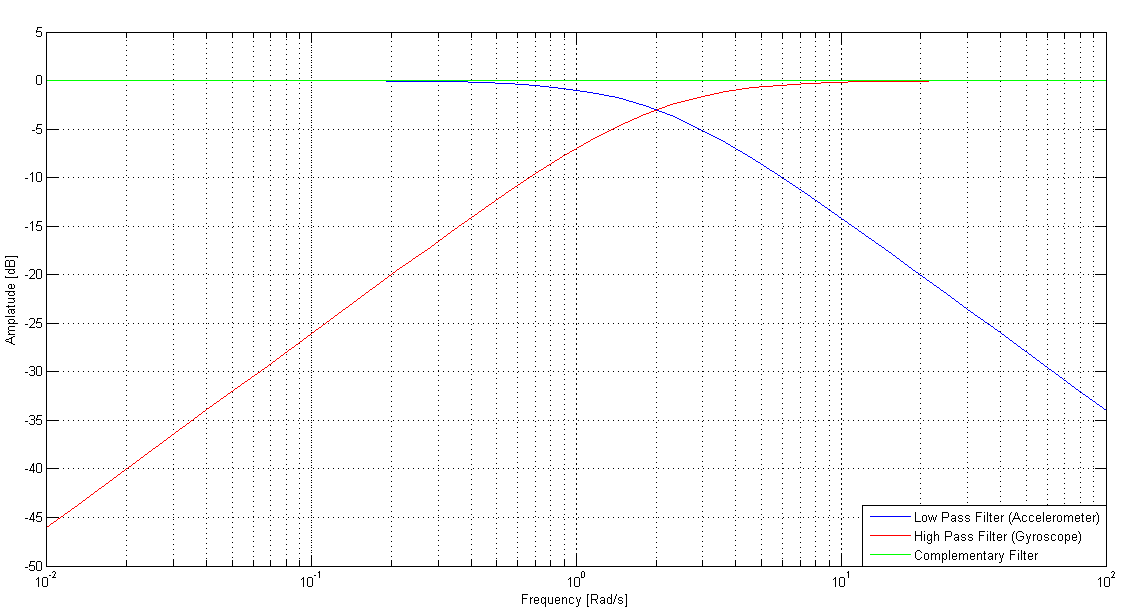
\includegraphics[width =0.7 \paperwidth]{\DocRoot/images/first_order_bode_plot}
	\caption{Bode plot of first order complementary filter}
	\label{Fig:bode first order com}
\end{figure}


Note as the orientation required for the control of the quad-rotor is in the \gls{ned} frame and as the sensor readings were in the \gls{bf} frame, a mapping was required to ensure the correct angles. These mappings which were presented in \eqref{Eq: angles from acc1}, \eqref{Eq: angleur velocity from gyro1} and\eqref{eq: filter order filter1}. These mappings allowed 
the high frequency components to be filtered so that an adequate estimation of the orientation could be achieved by means of a high-pass on gyroscope data:-
\begin{align}
	\dot{\gls{roll}}_{hp}  & =   \gls{wx} + S_{\gls{roll}}T_{\gls{pitch}}\gls{wy} + C_{\gls{roll}}T_{\gls{pitch}}\gls{wz}   - \frac{\gls{roll}_{hp}}{\tau} \\
	\dot{\gls{pitch}}_{hp} & =  C_{\gls{roll}}\gls{wy} - S_{\gls{roll}}\gls{wz} - \frac{\gls{pitch}_{hp}}{\tau}
\end{align}

By a similar mapping system the following low frequency components can be derived by means of a low-pass filter on the accelerometer:-

\begin{align}
	\dot{\gls{roll}}_{lp}  & =   \frac{1}{\tau}\left[\arctan\left(\frac{\gls{ay}}{\gls{ay}}\right) - \gls{roll}_{lp}\right]                      \\
	\dot{\gls{pitch}}_{lp} & =  \frac{1}{\tau}\left[\arctan\left(\frac{-\gls{ax}}{\sqrt{\gls{ay}^2+\gls{az}^2}}\right) - \gls{pitch}_{lp}\right]
\end{align}

\subsection{Difference Equations for first order filter}
Equation \ref{eq: filter order filter1} was emulated into the digital domain using Tustin's approximation to integration. Tustin's method was chosen as it ensures a stable mapping into the discrete domain (maps to inside the unit circle) if the continues function is stable.
\begin{equation}
	\begin{split}
		\gls{filterdata} [k] = \frac{1}{\gls{ts} + 2\tau}(\gls{ts} ( \gls{accdata} [k] + \gls{accdata} [k-1]  +  \tau(\gls{gyrodata} [k] + &\gls{gyrodata} [k-1])) \\ &-(\gls{ts} -2\tau)\gls{filterdata} [k-1] ) \label{eq: diff equation for the first order comp filter}
	\end{split}
\end{equation}


Equation \ref{eq: diff equation for the first order comp filter} was implemented on the micro-controller without the frame adjustments stated in \eqref{eq:acc simplified equation1} and \eqref{Eq: angleur velocity from gyro1}. These reductions were possible as the pitch (\gls{pitch}) and roll (\gls{roll}) angles were limited to $\pm 30^o$, these limitations allowed the trigonometric functions presented in \eqref{Eq: angleur velocity from gyro1} and \eqref{eq:acc simplified equation1} to be modeled as unity and \gls{pitch} or \gls{roll} for the $cos$ and $sin$ functions respectively. This was employed to reduce the sampling time of the critical control loops and can be easily added again if a faster micro-controller with a hardware \gls{fpu} \footnote{A micro-controller that has these requirements is the \textit{Tiva-C LaunchPad} which features a ARM Cortex-M4F which has a hardware \gls{fpu}} is used for the project in the future.  

The first order filter shown above was implemented both in Simulink and on the micro-controller along with the attitude controller. The filter was tuned in a similar method presented in algorithm \ref{Alg: auto tune of comp filter1} where the phase delay and \gls{rmse} weightings were adjusted until an adequate result was reached. Figure \ref{fig first order comp time and freq responce} compares the estimated pitch angle to the actual value. The results are adequate, but the gyroscope drift has not been fully eliminated and so another method of estimating the attitude of the quad-rotor was investigated. It was first decided to investigate a second order Complementary Filter. 

\begin{figure}[h]
	\centering
	\begin{subfigure}{0.32\textwidth}
		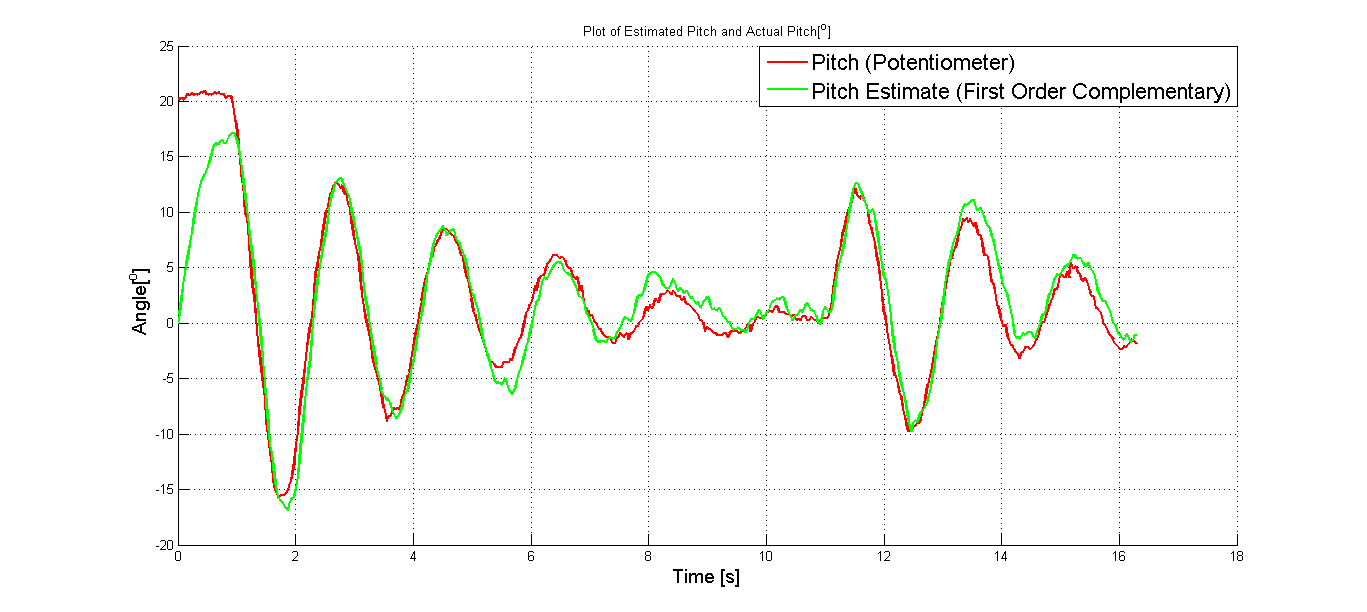
\includegraphics[width =0.36\paperwidth]{\DocRoot/images/comp_first_order_time}
		\caption{Time domain response of a first order Complementary Filter}
		\label{fg: Time domain comparison responce of the first order comp filter}
	\end{subfigure}%
	\hspace{3cm}
	\begin{subfigure}{0.32\textwidth}
		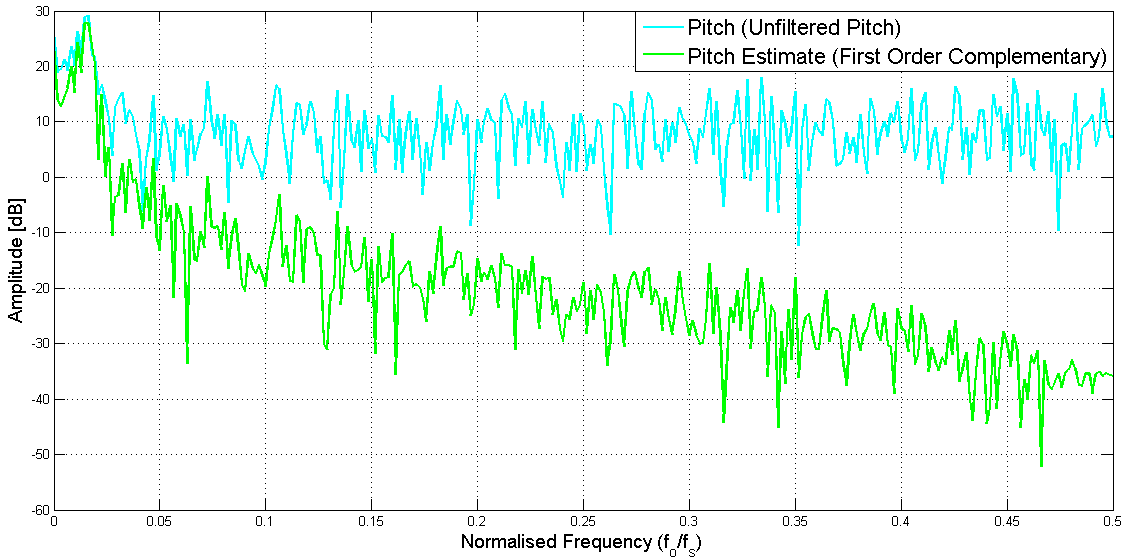
\includegraphics[width =0.36\paperwidth]{\DocRoot/images/comp_first_order_freq}
		\caption{Frequency domain response of a first order Complementary Filter}
		\label{fg: Frequency domain responce of the first order comp filter}
	\end{subfigure}
	
	\caption{Response of a first order complementary filter for $\tau = 0.5$ and ${\gls{ts}} = 30~\mathrm{ms}$ }
	\label{fig first order comp time and freq responce}
\end{figure}

\subsection{Second Order Complementary Filter}
As the drift on the gyroscope was still present after implementing the first order complementary filter on the micro-controller it was decided to implement a second order complementary filter similar to the one researched by Mahony \& Madgwick \cite{comp_filter_mit}. The filter presented in this section has two tuning parameters $K_p~\&~K_i$, this means that this filter is more versatile than the first order complementary filter which has only one tunning parameter $\tau$.



\begin{figure}[h]
	\begin{subfigure}[b]{0.32\textwidth}
		\resizebox{7.5cm}{3cm}
		{\begin{tikzpicture}[auto, thick, node distance=2cm, >=triangle 45]
				\draw
				% Drawing the blocks of first filter :	
				node at (0,0) [input,name=input1,thick,above]{}
				node at (3,0)[block] (lpf) {\Large $\frac{K_i + K_ps}{K_i +K_ps + s^2}$}
				node at (0,-2) [name=input2] {}
				node at (5.5,-2) [block](inte1) {\inte}
				node at (3,-2)[block] (hpf) {\Large $\frac{s^2}{K_i + K_ps +s^2}$}
				node at (7,-1)[sum={+}{}{+}{}] (suma1) {}
				node at (9,-1) [name=out] {};
				% Commands \draw with options like [->] must be written individually
				\draw[->](input1) -- node {$\gls{accdata}$} (lpf);
				\draw[->](input2) -- node {$\gls{gyrodata}$}(hpf);
				\draw[->](hpf) -- node {}(inte1);
				\draw[->](inte1) -| node {}(suma1);         %note the -| does the right angle
				\draw[->](lpf) -| node {}(suma1);
				\draw[->](suma1) -- node {$\gls{filterdata}$}(out);
			\end{tikzpicture}}
		\vspace{0.2cm}
		\caption{Block Diagram of Second Order Complementary Filter}
		\label{fig: Block Diagram of Second Order Complementary Filter}
	\end{subfigure}%
	\hspace{3cm}
	\begin{subfigure}[b]{0.32\textwidth}
		\resizebox{7.5cm}{3.5cm}{\begin{tikzpicture}[auto, thick, node distance=2cm, >=triangle 45]
				\draw
				% Drawing the blocks of first filter :
				node at (-0.3,0)     {$\gls{accdata}$}
				node at (0,0)      [input,name=input1,thick,above]{}
				node at (-0.3,-2.5)  {$\gls{gyrodata}$}
				node at (0,-2.5)   [input,name=input2,thick,above]{}
				
				node at (1,0)[sum={}{-}{+}{}] (sum1) {}
				node at (2,0) [joint] (joint1) {}
				node at (4,0) [block](inte1) {\inte}
				node at (6,0) [gain](ki){$K_i$}
				node at (4,2) [gain](kp){$K_p$}
				node at (7.5,0)[sum={+}{+}{}{}] (sum2) {}
				node at (8.5,0)[sum={}{-}{+}{}] (sum3) {}
				node at (10,0) [block](inte2) {\inte}
				node at (11,0) [joint] (joint2) {}
				node at (11.5,0) (out) {}
				node at (11.7,0)  {$\gls{filterdata}$};
				
				% Commands \draw with options like [->] must be written individually
				\draw[->](input1) -- node {}(sum1);
				\draw[->](sum1) -- node {} (inte1);
				\draw[->](joint1) |- node {} (kp);
				\draw[->](inte1) -- node {} (ki);
				\draw[->](ki) -- node {} (sum2);
				\draw[->](kp) -| node {} (sum2);
				\draw[->](input2) -| node {} (sum3);
				\draw[->](sum2) -- node {} (sum3);
				\draw[->](sum3) -- node {} (inte2);
				\draw[->](inte2) -- node {} (out);
				\draw(joint2) -- ++(0,-1.5) [->] -| node {} (sum1);
			\end{tikzpicture}}
		\caption{Feedback Block Diagram of Second Order Complementary Filter}
		\label{fig:Feedback Block Diagram of Second Order Complementary Filter2}
	\end{subfigure}
	\caption{Second Order Complementary Filter Block Diagrams}
	\label{fig: second order comp filter}
\end{figure}


The second order complementary filter described in figure \ref{fig: second order comp filter} can be defined over all frequencies by \eqref{eq: second order filter1}:-


\begin{equation}
	\gls{filterdata}=\underbrace{ {\frac{K_i + K_p s}{K_i + K_p s + s^2}}}_{\text{$G_1(s)$}}\gls{accdata} + \underbrace{\frac{s^2}{K_i+K_p s + s^2}}_{\text{$G_2(s)$}}\frac{1}{s}\gls{gyrodata}
	\label{eq: second order filter1}
\end{equation}

As can be seen from Figure \ref{Fig:bode sec order com} the filters presented in \eqref{eq: second order filter1} are complementary.   


\begin{figure}[h]
	\centering
	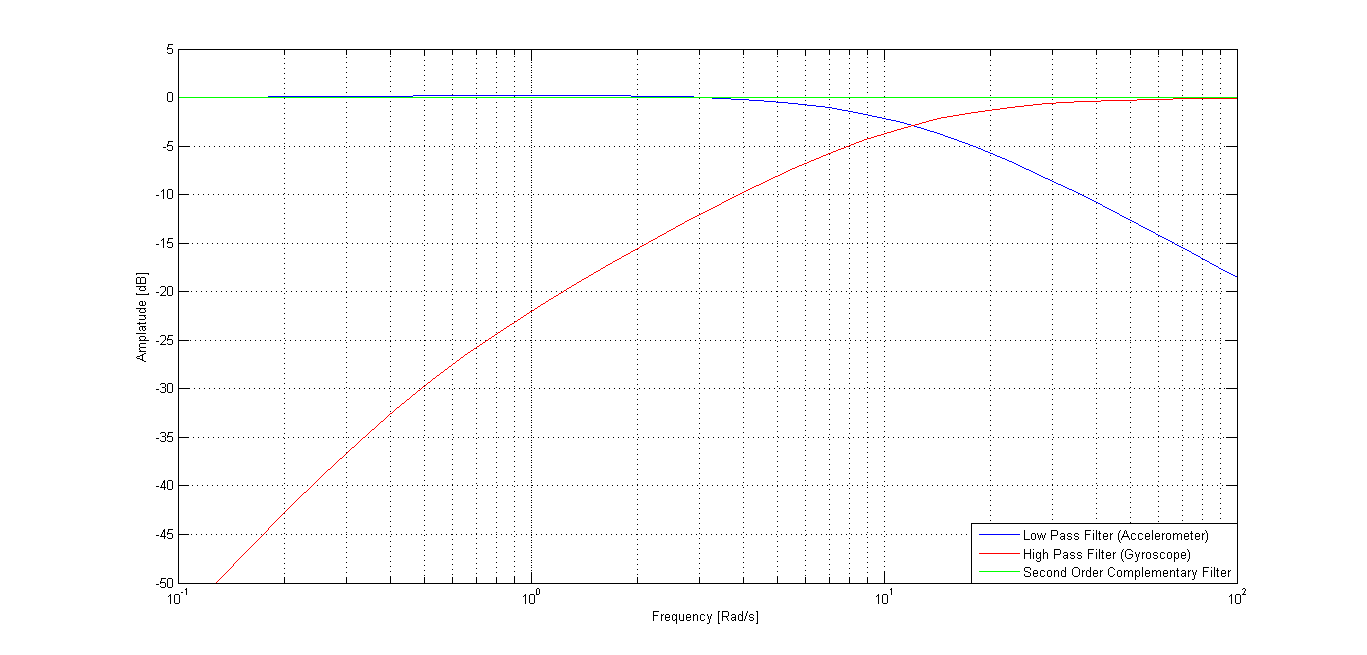
\includegraphics[width =0.8 \paperwidth]{\DocRoot/images/sec_order_bode_plot}
	\caption{Bode plot of a common second order complementary filter}
	\label{Fig:bode sec order com}
\end{figure}

Obviously, and not unexpectedly, this complementary filter is made from $2^{\mathrm{nd}}$ order filters. Note that the filter acting on the acceleration data actually consists of a low-pass plus a band-pass filter.

This result has interesting consequences. As the filters are $2^{\mathrm{nd}}$ order, the frequency response of the acceleration and gyroscope filters are characterized by the resonance frequency and damping factor

\begin{equation}
	\omega_0 = \sqrt{K_i}~~~~~~~ \xi = \frac{K_p}{2\sqrt{K_i}}
	\label{eq: second order comp filter ki and kp}
\end{equation}


The damping factor determines the overshoot at the resonance frequency. For manual tuning of this filter a flat frequency response can be achieved by setting $\xi \geq 1$ in \eqref{eq: second order comp filter ki and kp}. After doing this, one will get the following tuning criteria. 

\begin{equation}
	K_i \leq \frac{1}{4}K_p^2
\end{equation}
The results of this type of tuning can be seen in Figure \ref{fig sec order comp time and freq responce} and estimated the orientation of the quad-rotor to a certain degree, but as a whole was unsatisfactory. As a result two other methods of auto-tuning the filter were investigated, one which used a least squares and another which used a grid search. Before a grid based tuning approach could be implemented a discrete time version of the filter had to be created. 

Thus, to model the filter in MatLab $G_1(s)$ and $G_2(s)$ were arranged as follows:-
\begin{align}
	\chi_{hp} & = \frac{1}{s}\left[\gls{gyrodata} - \chi_{hp}\left({\frac{K_i}{s} + K_p}\right)\right] \label{Eq: second order comp high pass second1} \\
	\chi_{lp} & = \frac{1}{s}\left[(\gls{accdata} - \chi_{lp})\left({\frac{K_i}{s} + K_p}\right)\right] \label{Eq: second order comp low pass second1}
\end{align}


Note \eqref{Eq: second order comp high pass second1} and \eqref{Eq: second order comp low pass second1} can be combined to yield the following filter (as $\chi_{hp} + \chi_{lp} =  \gls{filterdata} $), which can also be modeled in MatLab.

\begin{equation}
	\gls{filterdata}  = \frac{1}{s}\left[\gls{gyrodata} +\left({\frac{K_i}{s} + K_p}\right)(\gls{filterdata}   - \gls{accdata})\right] \label{eq: comp filter equation used to tune comp filter1}
\end{equation}

\begin{figure}[h]
	\centering
	\begin{subfigure}{0.32\textwidth}
		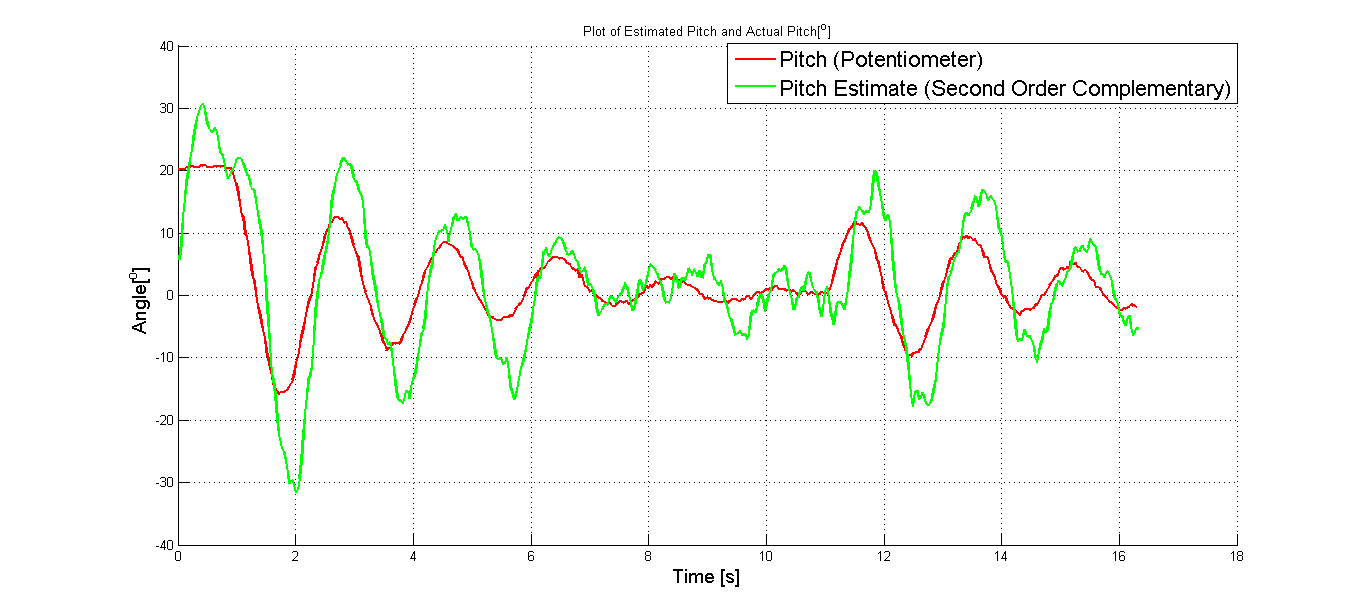
\includegraphics[width =0.38\paperwidth]{\DocRoot/images/comp_sec_time_man}
		\caption{Time domain response of a Second order Complementary Filter}
		\label{fg: Time domain comparison responce of the sec order comp filter}
	\end{subfigure}%
	\hspace{3cm}
	\begin{subfigure}{0.32\textwidth}
		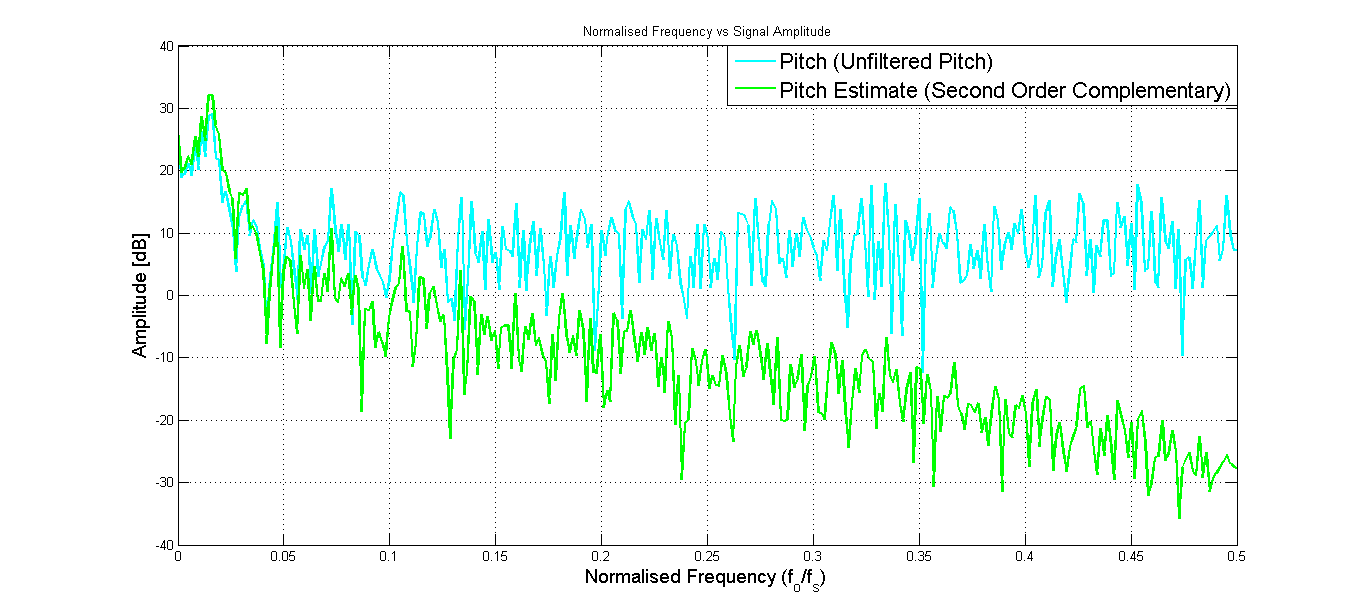
\includegraphics[width =0.38\paperwidth]{\DocRoot/images/comp_sec_fre_man}
		\caption{Frequency domain response of a Second order Complementary Filter}
		\label{fg: Frequency domain responce of the sec order comp filter}
	\end{subfigure}
	
	\caption{Response of a Second order complementary filter for $K_i = 25$, $K_p = 7$ and ${\gls{ts}} = 30~\mathrm{ms}$ }
	\label{fig sec order comp time and freq responce}
\end{figure}

\newpage
\subsection{Difference Equations for second order filter}
In order to implement the second order complementary filter on a micro-controller \eqref{Eq: second order comp high pass second1}and \eqref{Eq: second order comp low pass second1} were emulated into the digital domain using Tustin's method, which yielded the following equations:-
\begin{align}
	\chi_{hp}[k] & = \frac{1}{\eta + 4}\left(2\gls{ts} ( \gls{gyrodata} [k] - \gls{gyrodata} [k -2] ) - (\Gamma + 4)\chi_{hp}[k-2] - (\xi - 8)\chi_{hp}[k-1] \right) \label{Eq: second order comp high pass second difference eq1}                       \\
	\chi_{lp}[k] & = \frac{1}{\eta +4}\left(\Gamma \gls{accdata} [k-2] + \xi \gls{accdata} [k-1] + \eta \gls{accdata} [k] - (\Gamma + 4)\chi_{lp}[k-2] - (\xi - 8) \chi_{lp}[k - 1] \right) \label{Eq: second order comp low pass second difference eq1}
\end{align}


where:-

\begin{equation*}
	\eta = K_i\gls{ts}^2 + 2K_p\gls{ts};~~~ \Gamma = K_i\gls{ts}^2 - 2 K_p\gls{ts};~~~ \xi = 2K_i\gls{ts}^2
\end{equation*}

Before auto-tuning of the filter was implemented \eqref{Eq: second order comp high pass second difference eq1} and \eqref{Eq: second order comp low pass second difference eq1} where combined to give \eqref{Eq: full dfference equation for the second order filter1}. This was the equation that was used to tune the filter. Note \eqref{eq: comp filter equation used to tune comp filter1} could also be used to tune the filter, but when the filter is emulated there are distortions introduced by the emulation process.

\begin{multline}
	\gls{filterdata} [k] = \frac{1}{\eta +4}(\Gamma \gls{accdata} [k-2] + \xi \gls{accdata} [k-1] + \eta \gls{accdata} [k] + 2\gls{ts} ( \gls{gyrodata} [k] \\
	- \gls{gyrodata} [k -2] )   - (\Gamma + 4)\gls{filterdata} [k-2] - (\xi - 8) \gls{filterdata} [k - 1] ) \label{Eq: full dfference equation for the second order filter1}
\end{multline}

\section{Tuning of the Complementary Filter using Least Squares }
As a manual approach to tuning the second order filter yielded inadequate results, other methods of tuning the filter were investigated. One of the more useful approaches to tuning the filter was the least squares approach. Using \eqref{eq: comp filter equation used to tune comp filter1} one can tune the filter in the continuous domain and then emulate it across. This can be done by making the following assumption:-
\begin{equation}
	\gls{filterdata} = \gls{potangle}
\end{equation}
Where \gls{potangle} is the angle of the system as given by the potentiometer. In order to accomplish this  access to the rate of change of potentiometer angle as denoted as $\dot{\gls{potangle}}$. Hence, a method of tuning the filter as follows:-



\begin{align}
	\begin{split}
		\gls{potangle} &= \frac{1}{s}\left[ \gls{gyrodata} -\left(K_p + \frac{K_i}{s}\right) (\gls{potangle} - \gls{accdata})\right]\\
		\dot{\gls{potangle} }&= \left[ \gls{gyrodata} -\left(K_p + \frac{K_i}{s}\right) (\gls{potangle} - \gls{accdata})\right]\\
		\underbrace{\dot{\gls{potangle} } - \gls{gyrodata}}_{\text{$B_f$}}& = \underbrace{\left[(\gls{gyrodata} - \gls{potangle} ) + \frac{(\gls{gyrodata} - \gls{potangle} )}{s} \right] }_{\text{$A_f$}} \left[\begin{array}{c} K_p\\ K_i\end{array}\right] \label{eq: placer for leasr square eqaution1}
	\end{split}
\end{align}

Thus, using the equation developed in \eqref{eq: placer for leasr square eqaution1} one can tune a continuous time complementary filter of this form using the following:- 
\begin{equation}
	\left[\begin{array}{c} K_p\\ K_i\end{array}\right] = (A_f^\intercal A_f)^{-1}A_f^\intercal B_f \label{eq: tuning of complmentry filter in continues time least squares1}
\end{equation}

Note the method of tuning the filter as shown in \eqref{eq: tuning of complmentry filter in continues time least squares1} was done without a $\dot{\gls{potangle}}$ term. Instead a value was set for $(\gls{gyrodata} - \dot{\gls{potangle})}$ which was a valid approximation as the output of the gyroscope was low pass filtered on-chip with a first order filter which has a cutoff frequency of 100 \textit{Hz}. The results of this tuning method can be seen in Figure \ref{fig sec order comp time and freq responce least}


\begin{figure}[h]
	\centering
	\begin{subfigure}{0.32\textwidth}
		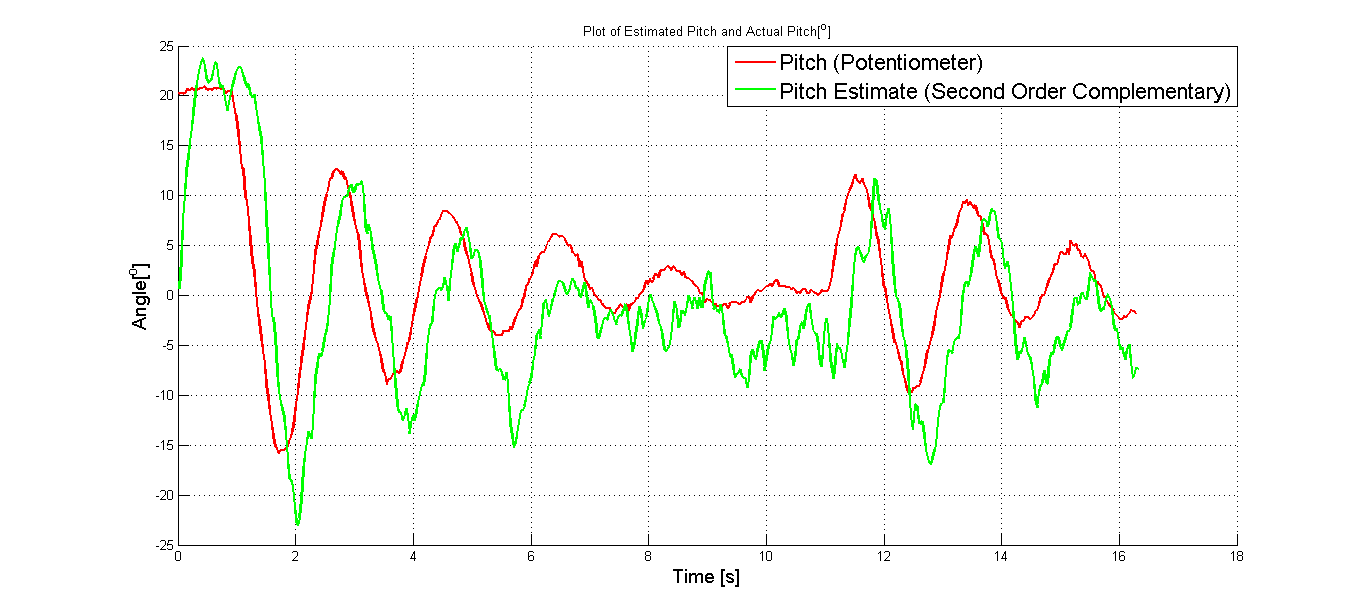
\includegraphics[width =0.38\paperwidth]{\DocRoot/images/comp_sec_time_auto}
		\caption{Time domain response of a Second order Complementary Filter}
		\label{fg: Time domain comparison responce of the sec order comp filter least}
	\end{subfigure}%
	\hspace{3cm}
	\begin{subfigure}{0.32\textwidth}
		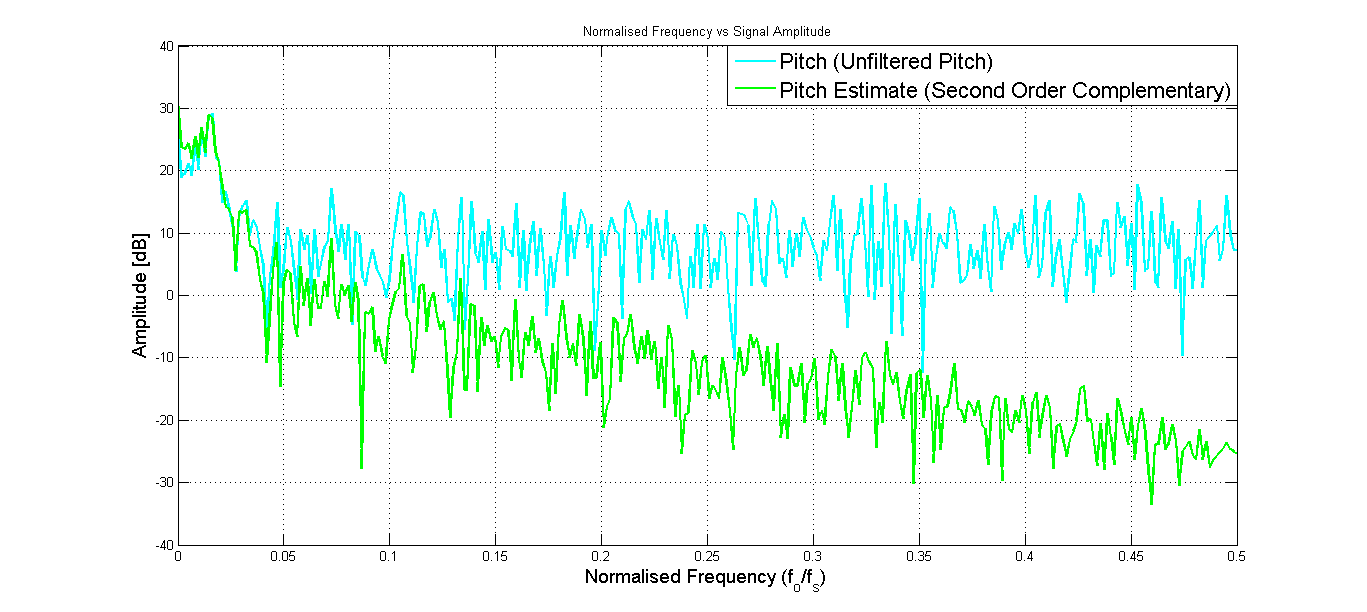
\includegraphics[width =0.38\paperwidth]{\DocRoot/images/comp_sec_fft_least}
		\caption{Frequency domain response of a Second order Complementary Filter}
		\label{fg: Frequency domain responce of the sec order comp filter least}
	\end{subfigure}
	
	\caption{Response of a Second order complementary filter for $K_i = 1.3265$, $K_p = 2.79322$ and ${\gls{ts}} = 30~\mathrm{ms}$ }
	\label{fig sec order comp time and freq responce least}
\end{figure}

\section{Self Tunning Algorithm for a Complementary Filter}

As the \enquote{actual} angle \gls{potangle} of the quad-rotor was known when tuning the filter it was decided to do a search using a \gls{rmse} \eqref{eq:rmse1}. A cross-correlation was done to find the delay between the filtered angle and the \enquote{actual} angle and remove when checking the \gls{rmse} term. This had the best results for the tuned filter and a trade off between lag\footnote{Note with this filter the lag can be set so it does not exceed the maximum allowable phase delay} and filtering could be set. Figure \ref{fig sec order comp time and freq responce auto}	proves that drift on the gyroscope has been removed, but the phase delay of the filtered signal has increased dramatical. 

\begin{equation}
	\gls{rmse} = \sqrt{\frac{\sum_{k = 1}^{n} (\gls{filterdata} -\gls{potangle})^2}{n}} \label{eq:rmse1}
\end{equation}

The cross-correlation function is defined in \eqref{eq: cross-correlation1} and is commonly used in signal processing to find the measure of time-lag between two signals.

\begin{equation}
	(f \star g)[n] = \sum_{m = -\infty}^{\infty} f^*[m]g[m+n] \label{eq: cross-correlation1}
\end{equation}



\begin{algorithm}
	\caption{Auto Tuning a Complementary Filter }\label{Alg: auto tune of comp filter1}
	\begin{algorithmic}[1]
		{	
			\renewcommand{\baselinestretch}{2.5}
			\Procedure{Grid search tuning of a Complementary Filter }{}
			\State Set max value for $K_p$, $K_i$, an \gls{rmse} value and the associated tolerance for the grid.
			
			
			
			\State {\color{white} .}
			\For {length($K_{p(it)}$)} \Comment{$K_{p(it)}$ an array of $K_p$ values to test}
			\State {\color{white} .}
			
			\For {length($K_{i(it)}$}  \Comment{$K_{i(it)}$ an array of $K_i$ values to test}
			\vspace{0.2cm}
			
			\State Calculate \gls{filterdata} the  filtered output using  \eqref{Eq: full dfference equation for the second order filter1}
			\vspace{0.2cm}
			
			\State Calculate Signal Delay of the Filtered output by means of equation \eqref{eq: cross-correlation1} \\ \hspace{2.5cm} by using \gls{filterdata} and \gls{potangle} as it's inputs.
			\vspace{0.2cm}
			\State Remove delay in filtered data by removing samples equal to  the value \\ \hspace{2.5cm}  returned by the previous line of code.
			\vspace{0.2cm}
			\State   Computer the \gls{rmse} value of the filtered signal using equation \eqref{eq:rmse1} \\ \hspace{2.5cm} and \gls{filterdata} \& \gls{potangle} as it's inputs.
			
			\State {\color{white} .}
			\If {(\gls{rmse}  < Previous Error)}
			\State $K_p$ = $K_{p(it)}$(i);
			\State $K_i$ = $K_{i(it)}$ (j);
			\State Previous Error = \gls{rmse};
			\EndIf
			\EndFor
			\EndFor
			
			\State {\color{white} .}
			
			\State \Return {$K_p$ \& $K_i$}
			\EndProcedure}
	\end{algorithmic}
\end{algorithm}

\begin{figure}[h]
	\centering
	\begin{subfigure}{0.32\textwidth}
		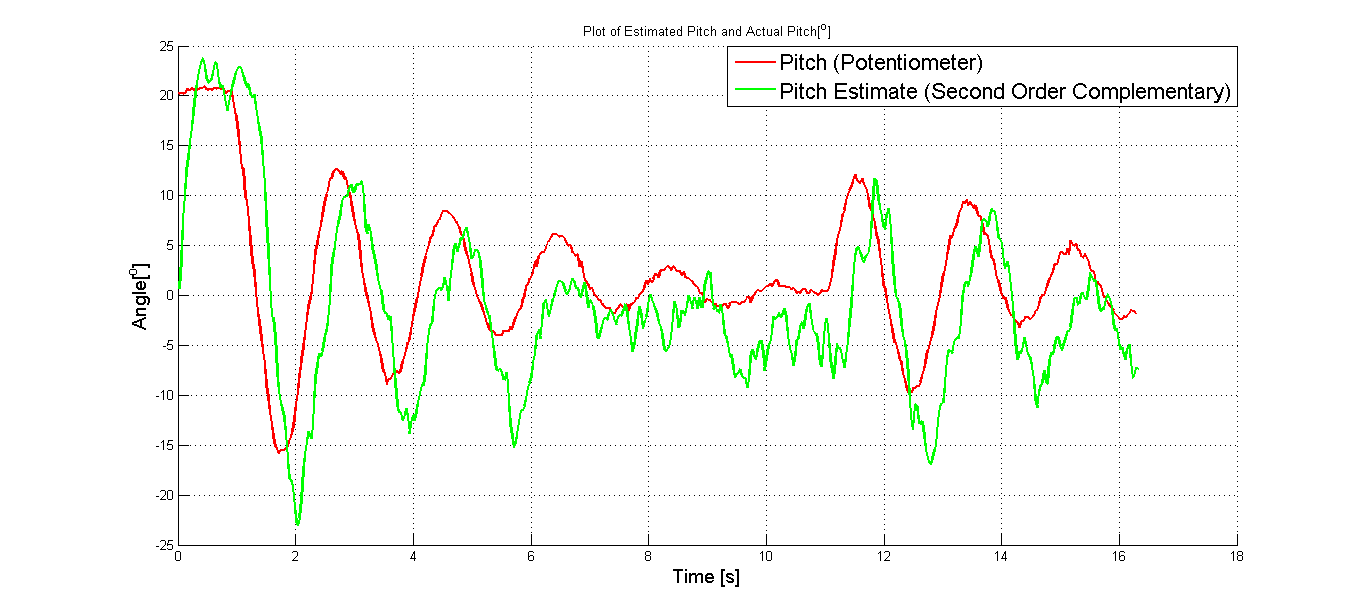
\includegraphics[width =0.38\paperwidth]{\DocRoot/images/comp_sec_time_auto}
		\caption{Time domain response of a Second order Complementary Filter}
		\label{fg: Time domain comparison responce of the sec order comp filter auto}
	\end{subfigure}%
	\hspace{3cm}
	\begin{subfigure}{0.32\textwidth}
		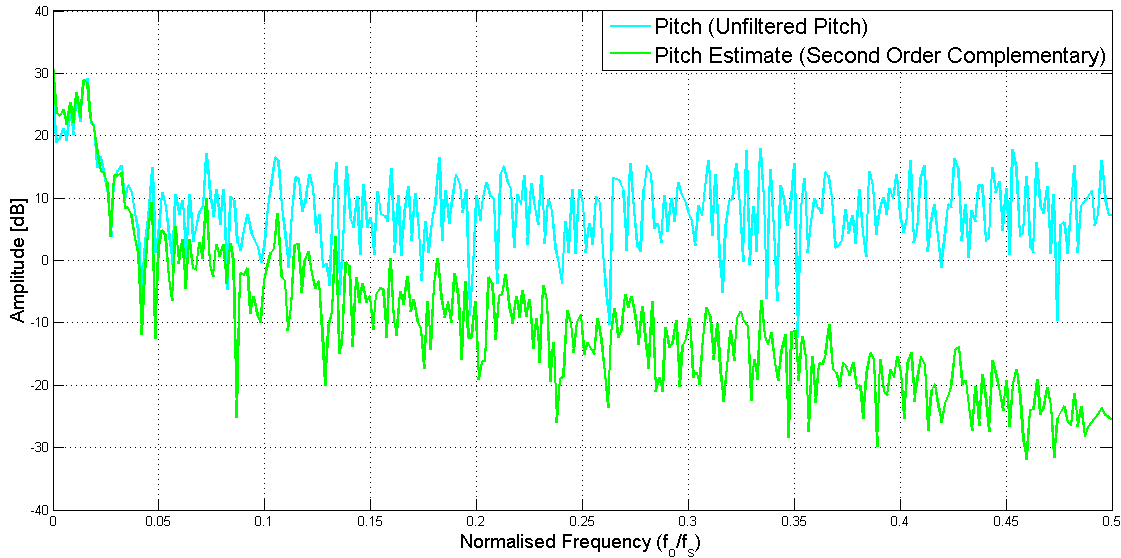
\includegraphics[width =0.38\paperwidth]{\DocRoot/images/comp_sec_fre_auto}
		\caption{Frequency domain response of a Second order Complementary Filter}
		\label{fg: Frequency domain responce of the sec order comp filter auto}
	\end{subfigure}
	
	\caption{Response of a Second order complementary filter for $K_i = 1.2802$, $K_p = 7.1919$ and ${\gls{ts}} = 30~\mathrm{ms}$ }
	\label{fig sec order comp time and freq responce auto}
\end{figure}

As can be seen from Figure \ref{fig sec order comp time and freq responce auto} the second order Complementary Filter removes the bias from the gyroscope, but there is a large delay introduced. Note there is less noise rejection in the second order filter. Hence, another filter was investigated which will be presented next.